% Source-faithful schematic draft. Coordinates satisfy x^2=4y exactly.
% source_id=src-bfaf1f0ca2f3b8edd4a2455d39b464722513d2bb05efe36769938f1f187729e5
% source_sha256=fca2f5abda4a5e4982176417bf2f33b6b248847bffb0dcd09ae089c4f6a85b6e; PDF p.2; Q22.
% Each pair has x_A*x_B=-4, so its chord passes through F=(0,1).
% Tangents use slope x/2; the A_n and B_n tangents meet at C_n.
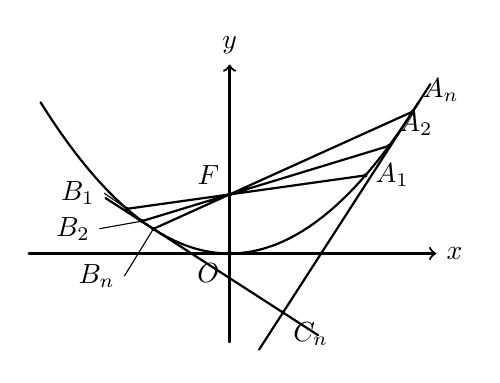
\begin{tikzpicture}[line cap=round,line join=round,thick,scale=0.75]
  \draw[->] (-3.4,0)--(3.5,0) node[right] {$x$};
  \draw[->] (0,-1.5)--(0,3.2) node[above] {$y$};
  \draw[domain=-3.2:3.2,samples=120] plot (\x,{\x*\x/4});
  \coordinate (O) at (0,0); \coordinate (F) at (0,1);
  \coordinate (A1) at (2.3,1.3225); \coordinate (B1) at (-1.73913,0.75614);
  \coordinate (A2) at (2.7,1.8225); \coordinate (B2) at (-1.48148,0.5487);
  \coordinate (An) at (3.1,2.4025); \coordinate (Bn) at (-1.29032,0.41623);
  \coordinate (Cn) at (0.90484,-1);
  % Focus chords A_i B_i, each passing through F.
  \draw (A1)--(B1) (A2)--(B2) (An)--(Bn);
  % Tangents at A_n and B_n: y=(x_n/2)x-x_n^2/4.
  \draw (0.5,-1.6275)--(An)--(3.4,2.8675);
  \draw (-2.1,0.9386)--(Bn)--(1.5,-1.3839);
  \fill (O) circle (1.2pt) node[below left] {$O$};
  \fill (F) circle (1.2pt) node[above left] {$F$};
  \foreach \p/\pos/\lab in {A1/right/A_1,A2/above right/A_2,An/above right/A_n,Cn/below right/C_n}
    \fill (\p) circle (1pt) node[\pos] {$\lab$};
  % Short leaders keep the three left labels distinct without moving points.
  \fill (B1) circle (1pt); \draw[thin] (B1)--(-2.12,1.02) node[left] {$B_1$};
  \fill (B2) circle (1pt); \draw[thin] (B2)--(-2.20,0.42) node[left] {$B_2$};
  \fill (Bn) circle (1pt); \draw[thin] (Bn)--(-1.78,-0.38) node[left] {$B_n$};
\end{tikzpicture}
